\section{Loss Systems}
There are multiple ways of measuring the quality of the bounding box that is produced by the model, the most used is of course the \gls{iou} or Jaccard Index. However, the \gls{iou} is more akin to a measure of \textit{how good} a bounding box is : an excellent bounding box will have an \gls{iou} close to 1. However, the \gls{iou} does not indicate \textit{how bad} a bounding box is: if there is no intersection between the bounding box and the ground truth, the \gls{iou} will of course be 0. But this means that bad bounding box that is close to the ground truth will have the same score as a \textit{very bad} bounding box that is far away from the ground truth. Recent work have been done to address this issue, and is presented here.

\subsection{GIoU, DIoU and CIoU}\label{ious}
\textbf{Generalized Intersection over Union Loss}: an improvement on the traditional Intersection over Union performance metric would be used to more accurately measure the accuracy of the bounding boxes. The \gls{giou} is defined as follows:

\begin{equation}
	GIoU = 1 -  IoU + \frac{area(B_{GT} \cup B_{PT})}{area(B_{EC})}
\label{eq:GIoU}
\end{equation}

With IoU being defined in Equation~\ref{eq:iou}

\begin{equation}\label{eq:iou}
	IoU = \frac{area(B_{GT} \cap B_{PT})}{area(B_{GT} \cup B_{PT})}
\end{equation}

In those equations, $B_{GT}$ represents the bounding box ground truth, $B_{PT}$ represents the predicted bounding box and $B_{EC}$ represents the smallest enclosing box of $B_{GT}$ and $B_{PT}$.

\begin{figure}[h!]
\begin{subfigure}{.5\textwidth}
  \centering
  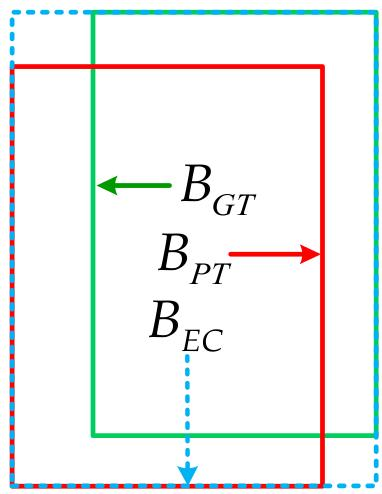
\includegraphics[width=.5\textwidth]{overlappingBox.jpg}  
  \caption{Two intersecting bounding boxes}
  \label{fig:sub-first}
\end{subfigure}
\begin{subfigure}{.5\textwidth}
  \centering
  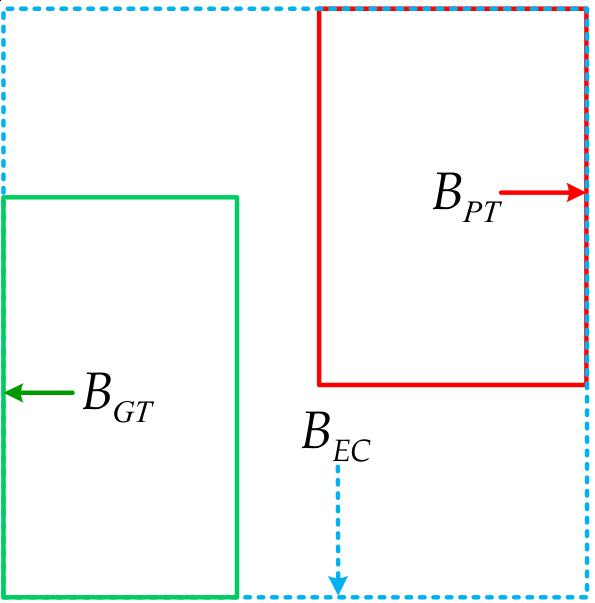
\includegraphics[width=.6\linewidth]{nonoverlappingBox.jpg}  
  \caption{Two non-overlapping bounding boxes}
  \label{fig:sub-second}
\end{subfigure}
	\caption[Bounding boxes overlap cases]{Illustration showing the two cases of bounding box position: intersecting and non-overlapping. The rectangle enclosed by a green solid line denotes the ground truth $B_{GT}$; the predicted box $B_{PT}$ is denoted by a red solid line, and the smallest enclosing box $B_{EC}$ is denoted by a blue dashed line.}
\label{fig:giou}
\end{figure}


The \gls{giou} loss is a better measure of the quality of the predicted bounding box. Qian \textit{et al.} also presents a new loss system that has a stronger gradient when the predicted bounding box is farther away to the truth. This loss system is shown in Equation~\ref{eq:giouLoss}

\begin{equation}\label{eq:giouLoss}
	\mathcal{L}_{GIoU} = 2 \times log_2 - 2 \times log(1 + GIoU)
\end{equation}
In Zheng \textit{et al.}\cite{diou} the general \gls{iou} loss is defined as follows:
\begin{equation}
	\mathcal{L} = 1 - IoU + \mathcal{R}(B_{GT}, B_{PT})
\end{equation}
Where  $\mathcal{R}(B_{GT}, B_{PT})$ is a penalty term for the predicted box and ground truth. The authors then design a specialised penalty based on this formula.

\textbf{The Distance IoU Loss} is defined as follows:
\begin{equation}
	\mathcal{L} = 1 - IoU + \frac {\rho^2(B_{GT}, B_{PT})}{c^2}
	\label{eq:diouLoss}
\end{equation}

Here, $b_{GT}, b_{PT}$ represents the center point of the ground truth bounding box and predicted box respectively, $\rho(\cdot)$ is the Euclidean distance and $c$ is the diagonal length of the smallest enclosing box covering the two boxes \textit{i.e.} $B_{EC}$.

\textbf{The Complete IoU Loss} incorporate the \gls{diou} and add another term which forces aspect ratio consistency. The \gls{ciou} is defined as follows:
\begin{equation}
	\mathcal{L} = 1 - IoU + \frac {\rho^2(B_{GT}, B_{PT})}{c^2} + \alpha v 
	\label{eq:ciouLoss}
\end{equation}
Where $\alpha$ is a positive trade-off parameters. $v$ measures the consistency of aspect ratios and is defined as follows.

\begin{equation}
	v = \frac{4}{\pi}(\arctan[\frac{w_{GT}}{h_{GT}}] -    \arctan[\frac{w_{PT}}{h_{PT}}])^2
	\label{eq:AspectRatio}
\end{equation}

Finally the trade-off parameter $\alpha$ is defined as follows:
\begin{equation}
	\alpha = \frac{v}{1 - IoU + v}
\end{equation}

The \gls{ciou} loss and the \gls{diou} both obtain \gls{ap} improvements up to $3.14 \%$ on a FasterR-CNN\cite{FasterRCNN} model trained on the COCO\cite{msCOCO} dataset, up to $2.92 \%$ on a SSD\cite{ssd} model also trained on COCO.

\subsection{Loss flooding}
In a recent paper by Ishida \textit{et al.}\cite{ishida2020}, a new kind of regularization is presented, where \textbf{the model is prevented from reaching a zero training loss, even though it has zero training error}. This technique, called \textit{flooding} intentionally prevents further reduction of he training loss when it reaches a certain low value: the \textit{flooding level}. This approach makes the loss move around the flooding level by doing gradient descent if the loss is above the flooding level, but gradient ascent if it is below. This technique allows the network to obtain better generalization results and is very easily implementable.

\begin{figure}[H]
	\begin{subfigure}[t]{.24\textwidth}
  \centering
  % include first image
  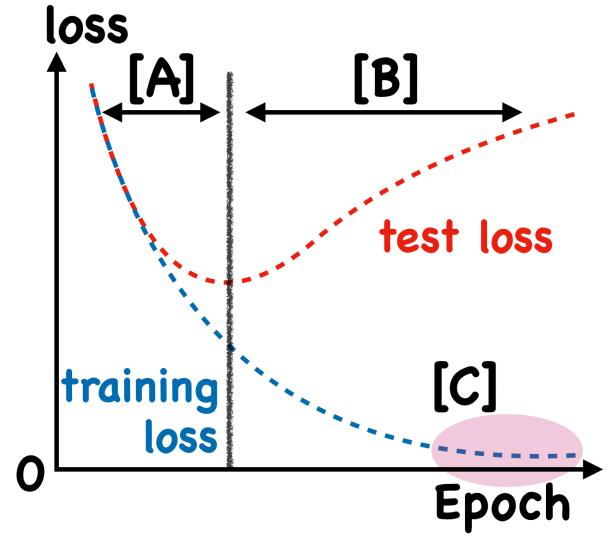
\includegraphics[width=\linewidth]{noLossA}  
  \caption{Without Flooding}
  \label{fig:lossA}
\end{subfigure}
	\begin{subfigure}[t]{.24\textwidth}
  \centering
  % include second image
  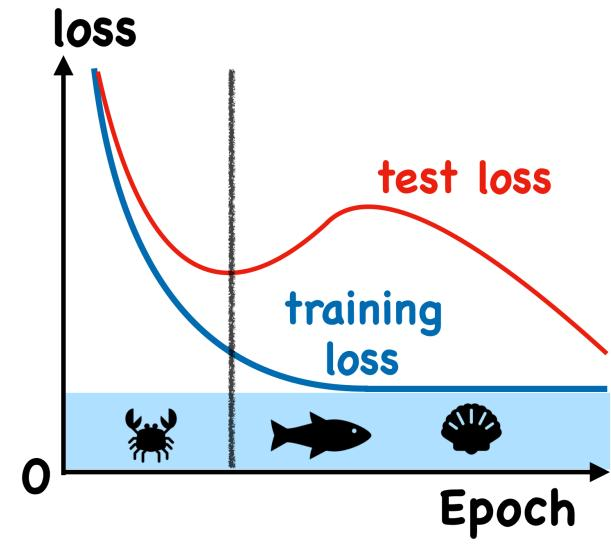
\includegraphics[width=\linewidth]{noLossB}  
  \caption{With Flooding}
  \label{fig:lossB}
\end{subfigure}
	\begin{subfigure}[t]{.24\textwidth}
  \centering
  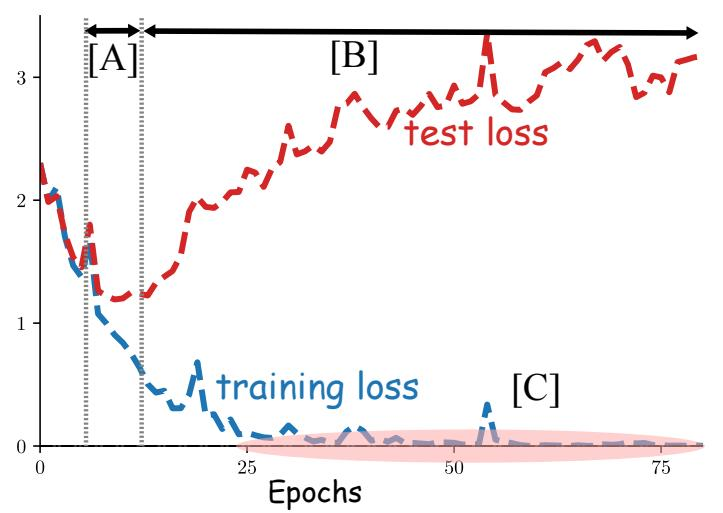
\includegraphics[width=\linewidth]{noLossC}  
  \caption{CIFAR-10 without flooding}
  \label{fig:lossC}
\end{subfigure}
	\begin{subfigure}[t]{.24\textwidth}
  \centering
  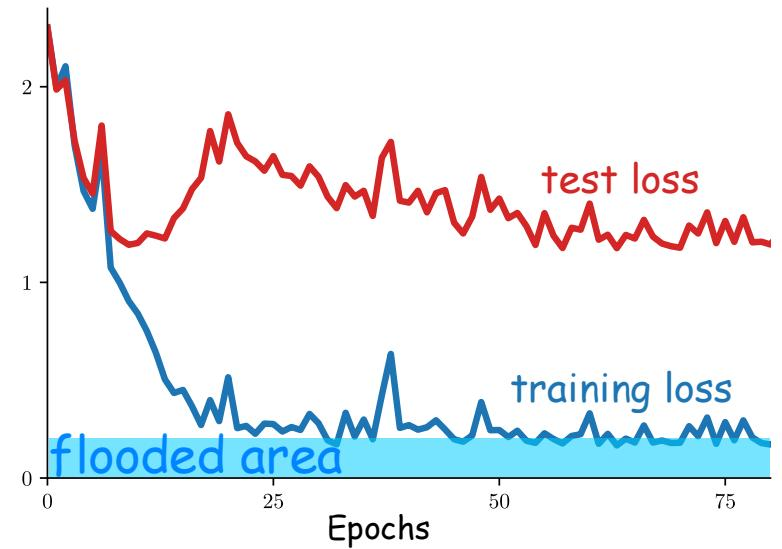
\includegraphics[width=\linewidth]{noLossD}  
  \caption{CIFAR-10 with flooding}
  \label{fig:lossD}
\end{subfigure}
	\caption[Loss flooding]{Subfigure (a) shows the different regime during which a network first learns, then overfit. During [A], the network learns correctly, and both the training loss and the test loss decreases. During [B] the training loss continues to decreases, but the test loss increases; this is overfitting. In [C] the training loss is nearly zero. The authors show a way to avoid [C] by flooding the bottom area, forcing the loss to stay around a constant, which leads to a decreasing test loss. This is seen in (b) and (c) on the CIFAR-10 dataset}
\label{fig:flooding}
\end{figure}

By letting the loss constant, the model hopefully drift towards a subspace where the loss landscape is flat, leading to better generalization. The authors tested this approach with various datasets, namely MNIST\cite{mnist}, Fashion-MNIST\cite{fashionMNIST}, CIFAR-10\cite{cifar} and often obtained better results and in nearly every datasets, suggesting this approach is effective. Considering the ease of implementation, the lack of performance degradation and the possible improvements on performance, this technique could be very worthwhile.

\section{Training methodology}
First, a non modified YOLOv4 model, using the original architecture has been trained on the dataset, and will serve as a baseline, along with the Fast RCNN model trained by Verschoof-van der Vaart and Lambers\cite{wouter2019}. This will allow us to effectively quantify the improvements or deteriorations in performance between the model themselves. 

We trained each model on the same dataset, for 10000 epochs. Most trainings were done using already pretrained weights used for detections on the COCO dataset, but some trainings were done using a completely untrained model. For every model, the best version of the weights were selected, based on the \gls{map}. Some models were also trained with defaults anchors, and with anchors computed specifically for the dataset, to see the impact of this modification.


